\documentclass[journal,12pt]{IEEEtran}
\usepackage{longtable}
\usepackage{setspace}
\usepackage{gensymb}
\singlespacing
\usepackage[cmex10]{amsmath}
\newcommand\myemptypage{
	\null
	\thispagestyle{empty}
	\addtocounter{page}{-1}
	\newpage
}
\usepackage{amsthm}
\usepackage{mdframed}
\usepackage{mathrsfs}
\usepackage{txfonts}
\usepackage{stfloats}
\usepackage{bm}
\usepackage{cite}
\usepackage{cases}
\usepackage{subfig}

\usepackage{longtable}
\usepackage{multirow}

\usepackage{enumitem}
\usepackage{mathtools}
\usepackage{steinmetz}
\usepackage{tikz}
\usepackage{circuitikz}
\usepackage{verbatim}
\usepackage{tfrupee}
\usepackage[breaklinks=true]{hyperref}
\usepackage{graphicx}
\usepackage{tkz-euclide}

\usetikzlibrary{calc,math}
\usepackage{listings}
    \usepackage{color}                                            %%
    \usepackage{array}                                            %%
    \usepackage{longtable}                                        %%
    \usepackage{calc}                                             %%
    \usepackage{multirow}                                         %%
    \usepackage{hhline}                                           %%
    \usepackage{ifthen}                                           %%
    \usepackage{lscape}     
\usepackage{multicol}
\usepackage{chngcntr}

\DeclareMathOperator*{\Res}{Res}

\renewcommand\thesection{\arabic{section}}
\renewcommand\thesubsection{\thesection.\arabic{subsection}}
\renewcommand\thesubsubsection{\thesubsection.\arabic{subsubsection}}

\renewcommand\thesectiondis{\arabic{section}}
\renewcommand\thesubsectiondis{\thesectiondis.\arabic{subsection}}
\renewcommand\thesubsubsectiondis{\thesubsectiondis.\arabic{subsubsection}}


\hyphenation{op-tical net-works semi-conduc-tor}
\def\inputGnumericTable{}                                 %%

\lstset{
%language=C,
frame=single, 
breaklines=true,
columns=fullflexible
}
\begin{document}
\onecolumn

\newtheorem{theorem}{Theorem}[section]
\newtheorem{problem}{Problem}
\newtheorem{proposition}{Proposition}[section]
\newtheorem{lemma}{Lemma}[section]
\newtheorem{corollary}[theorem]{Corollary}
\newtheorem{example}{Example}[section]
\newtheorem{definition}[problem]{Definition}

\newcommand{\BEQA}{\begin{eqnarray}}
\newcommand{\EEQA}{\end{eqnarray}}
\newcommand{\define}{\stackrel{\triangle}{=}}
\bibliographystyle{IEEEtran}
\raggedbottom
\setlength{\parindent}{0pt}
\providecommand{\mbf}{\mathbf}
\providecommand{\pr}[1]{\ensuremath{\Pr\left(#1\right)}}
\providecommand{\qfunc}[1]{\ensuremath{Q\left(#1\right)}}
\providecommand{\sbrak}[1]{\ensuremath{{}\left[#1\right]}}
\providecommand{\lsbrak}[1]{\ensuremath{{}\left[#1\right.}}
\providecommand{\rsbrak}[1]{\ensuremath{{}\left.#1\right]}}
\providecommand{\brak}[1]{\ensuremath{\left(#1\right)}}
\providecommand{\lbrak}[1]{\ensuremath{\left(#1\right.}}
\providecommand{\rbrak}[1]{\ensuremath{\left.#1\right)}}
\providecommand{\cbrak}[1]{\ensuremath{\left\{#1\right\}}}
\providecommand{\lcbrak}[1]{\ensuremath{\left\{#1\right.}}
\providecommand{\rcbrak}[1]{\ensuremath{\left.#1\right\}}}
\theoremstyle{remark}
\newtheorem{rem}{Remark}
\newcommand{\sgn}{\mathop{\mathrm{sgn}}}
\providecommand{\abs}[1]{\left\vert#1\right\vert}
\providecommand{\res}[1]{\Res\displaylimits_{#1}} 
\providecommand{\norm}[1]{\left\lVert#1\right\rVert}
%\providecommand{\norm}[1]{\lVert#1\rVert}
\providecommand{\mtx}[1]{\mathbf{#1}}
\providecommand{\mean}[1]{E\left[ #1 \right]}
\providecommand{\fourier}{\overset{\mathcal{F}}{ \rightleftharpoons}}
%\providecommand{\hilbert}{\overset{\mathcal{H}}{ \rightleftharpoons}}
\providecommand{\system}{\overset{\mathcal{H}}{ \longleftrightarrow}}
	%\newcommand{\solution}[2]{\textbf{Solution:}{#1}}
\newcommand{\solution}{\noindent \textbf{Solution: }}
\newcommand{\cosec}{\,\text{cosec}\,}
\providecommand{\dec}[2]{\ensuremath{\overset{#1}{\underset{#2}{\gtrless}}}}
\newcommand{\myvec}[1]{\ensuremath{\begin{pmatrix}#1\end{pmatrix}}}
\newcommand{\mydet}[1]{\ensuremath{\begin{vmatrix}#1\end{vmatrix}}}
\numberwithin{equation}{subsection}

\makeatletter
\@addtoreset{figure}{problem}
\makeatother
\let\StandardTheFigure\thefigure
\let\vec\mathbf

\renewcommand{\thefigure}{\theproblem}

\def\putbox#1#2#3{\makebox[0in][l]{\makebox[#1][l]{}\raisebox{\baselineskip}[0in][0in]{\raisebox{#2}[0in][0in]{#3}}}}
     \def\rightbox#1{\makebox[0in][r]{#1}}
     \def\centbox#1{\makebox[0in]{#1}}
     \def\topbox#1{\raisebox{-\baselineskip}[0in][0in]{#1}}
     \def\midbox#1{\raisebox{-0.5\baselineskip}[0in][0in]{#1}}
\vspace{3cm}
\title{Assignment 11}
\author{Sachinkumar Dubey - EE20MTECH11009}
\maketitle
\bigskip
\renewcommand{\thefigure}{\theenumi}
\renewcommand{\thetable}{\theenumi}
%
Download the latex-tikz codes from 
%
\begin{lstlisting}
https://github.com/sachinomdubey/Matrix-theory/Assignment11
\end{lstlisting}
\section{\textbf{Problem}}
(UGC-dec2017,105) : \\
%
Consider a Markov chain with five states $\{1,2,3,2,5\}$ and transition matrix
\begin{align}
    P=\myvec{\frac{1}{2} & 0 & 0 & \frac{1}{2} & 0\\
            0 & \frac{1}{7} & 0 & 0&\frac{6}{7}\\
              \frac{1}{5} & \frac{1}{5} & \frac{1}{5} & \frac{1}{5} & \frac{1}{5}\\ \frac{1}{3} & 0 & 0 & \frac{2}{3} & 0 \\
              0 & \frac{5}{8} & 0 & 0 & \frac{3}{8}}
\end{align}
Which of the following are true?\\
\begin{enumerate}
\item 3 and 1 are in the same communicating class
\item 1 and 4 are in the same communicating class
\item 4 and 2 are in the same communicating class
\item 2 and 5 are in the same communicating class
\end{enumerate}
\section{\textbf{Definition and Result used}}
\begin{longtable}{|l|l|}
	\hline
	\multirow{3}{*}{Accessibility of states} 
	& \\
	& We say that state $j$ is accessible from state $i$, written as $i \rightarrow j$, if $p^{(n)}_{ij}>0$\\ in Markov's chain
	& for some n. Every state is accessible from itself since $p^{(0)}_{ii}=1$\\
	&\\
	\hline
	\multirow{3}{*}{Communication between} & \\
	& Two states $i$ and $j$ are said to communicate, written as $i\leftrightarrow j$, if they\\ states
	& are accessible from each other. In other words,\\
	&\\
  	& \qquad \qquad  \qquad $i \leftrightarrow j  \;  \textrm{ means } \;  i \rightarrow j  \textrm{ and }  j \rightarrow i.$ \\
    	& \\
    	\hline
    	\multirow{3}{*}{Communicating class} & \\
	& For each Markov chain, there exists a unique decomposition of the \\
	& state space $S$ into a sequence of disjoint subsets $C_1, C_2, . . .,$\\
	&\\
    	&  \qquad \qquad  \qquad$S=\bigcup_{i=1}^{\infty}C_i$\\
    	&\\
    	& in which each subset has the property that all states within it communicate.\\
    	& Each such subset is called a communication class of the Markov chain.\\
    	&\\
    \hline
\end{longtable}
\newpage
\section{\textbf{Solution}}
	\begin{longtable}{|l|l|}
		\hline
		\multirow{3}{*}{Drawing Transition diagram} 
		& \\
		& 
		
		
\tikzset{every picture/.style={line width=0.75pt}} %set default line width to 0.75pt        
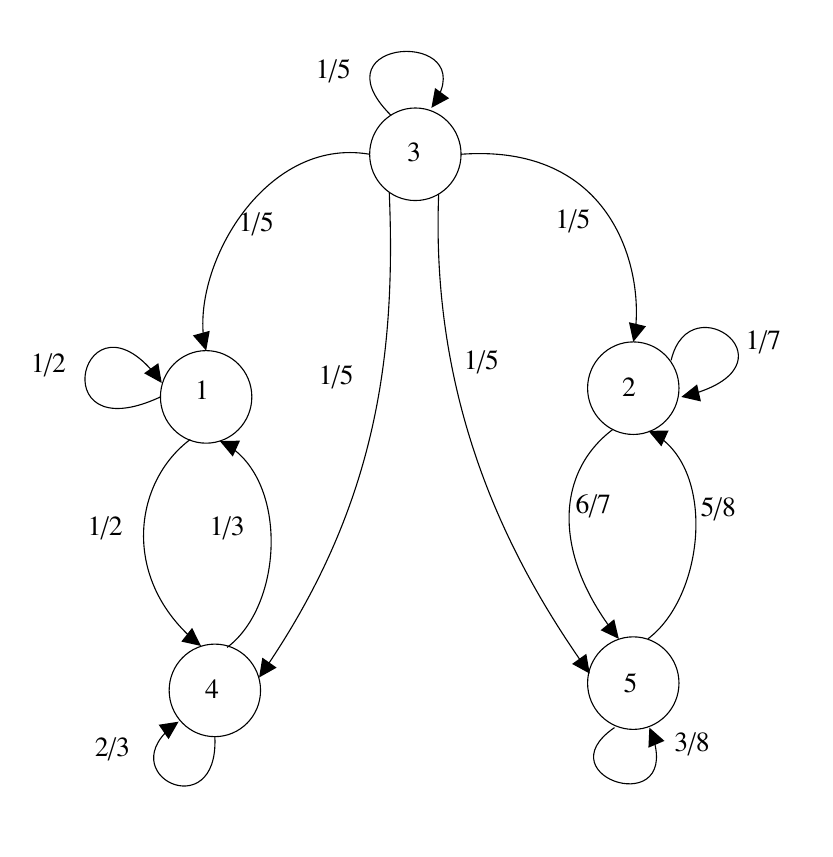
\begin{tikzpicture}[x=0.75pt,y=0.75pt,yscale=-0.7,xscale=0.7]
%uncomment if require: \path (0,714); %set diagram left start at 0, and has height of 714
%Shape: Ellipse [id:dp29836895541013164] 
\draw   (286,156.85) .. controls (286,139.26) and (300.08,125) .. (317.45,125) .. controls (334.82,125) and (348.9,139.26) .. (348.9,156.85) .. controls (348.9,174.44) and (334.82,188.7) .. (317.45,188.7) .. controls (300.08,188.7) and (286,174.44) .. (286,156.85) -- cycle ;
%Shape: Ellipse [id:dp4858180433459096] 
\draw   (142,323.85) .. controls (142,306.26) and (156.08,292) .. (173.45,292) .. controls (190.82,292) and (204.9,306.26) .. (204.9,323.85) .. controls (204.9,341.44) and (190.82,355.7) .. (173.45,355.7) .. controls (156.08,355.7) and (142,341.44) .. (142,323.85) -- cycle ;
%Shape: Ellipse [id:dp10893001214881792] 
\draw   (436,317.85) .. controls (436,300.26) and (450.08,286) .. (467.45,286) .. controls (484.82,286) and (498.9,300.26) .. (498.9,317.85) .. controls (498.9,335.44) and (484.82,349.7) .. (467.45,349.7) .. controls (450.08,349.7) and (436,335.44) .. (436,317.85) -- cycle ;
%Shape: Ellipse [id:dp31584444241771226] 
\draw   (148,525.85) .. controls (148,508.26) and (162.08,494) .. (179.45,494) .. controls (196.82,494) and (210.9,508.26) .. (210.9,525.85) .. controls (210.9,543.44) and (196.82,557.7) .. (179.45,557.7) .. controls (162.08,557.7) and (148,543.44) .. (148,525.85) -- cycle ;
%Shape: Ellipse [id:dp6845584977543557] 
\draw   (436,520.85) .. controls (436,503.26) and (450.08,489) .. (467.45,489) .. controls (484.82,489) and (498.9,503.26) .. (498.9,520.85) .. controls (498.9,538.44) and (484.82,552.7) .. (467.45,552.7) .. controls (450.08,552.7) and (436,538.44) .. (436,520.85) -- cycle ;
%Curve Lines [id:da40673715992947246] 
\draw    (212.24,513.63) .. controls (288.82,402.26) and (304.45,300.14) .. (299.5,183.32) ;
\draw [shift={(209.9,517)}, rotate = 304.9] [fill={rgb, 255:red, 0; green, 0; blue, 0 }  ][line width=0.08]  [draw opacity=0] (12.5,-6.01) -- (0,0) -- (12.5,6.01) -- cycle    ;
%Curve Lines [id:da5133467038577342] 
\draw    (172.69,288.89) .. controls (161.52,237.16) and (212.5,144.11) .. (286,156.85) ;
\draw [shift={(173.45,292)}, rotate = 254.65] [fill={rgb, 255:red, 0; green, 0; blue, 0 }  ][line width=0.08]  [draw opacity=0] (12.5,-6.01) -- (0,0) -- (12.5,6.01) -- cycle    ;
%Curve Lines [id:da008345831811055193] 
\draw    (167.44,493.28) .. controls (114.6,449.49) and (123.1,382.7) .. (162.5,353.15) ;
\draw [shift={(169.9,495.27)}, rotate = 218.21] [fill={rgb, 255:red, 0; green, 0; blue, 0 }  ][line width=0.08]  [draw opacity=0] (12.5,-6.01) -- (0,0) -- (12.5,6.01) -- cycle    ;
%Curve Lines [id:da5634268603548509] 
\draw    (435.25,511.14) .. controls (385.72,441.07) and (327.59,334.04) .. (333.5,184.32) ;
\draw [shift={(437.5,514.32)}, rotate = 234.46] [fill={rgb, 255:red, 0; green, 0; blue, 0 }  ][line width=0.08]  [draw opacity=0] (12.5,-6.01) -- (0,0) -- (12.5,6.01) -- cycle    ;
%Curve Lines [id:da4259073730032066] 
\draw    (187.9,496.27) .. controls (227.3,466.72) and (230.27,378.53) .. (185,355.28) ;
\draw [shift={(182.9,354.27)}, rotate = 384.44] [fill={rgb, 255:red, 0; green, 0; blue, 0 }  ][line width=0.08]  [draw opacity=0] (12.5,-6.01) -- (0,0) -- (12.5,6.01) -- cycle    ;
%Curve Lines [id:da6577514807411684] 
\draw    (468.08,283.01) .. controls (475.64,242.78) and (457.71,148.87) .. (348.9,156.85) ;
\draw [shift={(467.45,286)}, rotate = 283.29] [fill={rgb, 255:red, 0; green, 0; blue, 0 }  ][line width=0.08]  [draw opacity=0] (12.5,-6.01) -- (0,0) -- (12.5,6.01) -- cycle    ;
%Curve Lines [id:da329541870026538] 
\draw    (142,323.85) .. controls (58.35,362.99) and (88.88,241.85) .. (141.3,312.08) ;
\draw [shift={(142.9,314.27)}, rotate = 234.51] [fill={rgb, 255:red, 0; green, 0; blue, 0 }  ][line width=0.08]  [draw opacity=0] (12.5,-6.01) -- (0,0) -- (12.5,6.01) -- cycle    ;
%Curve Lines [id:da3393212160499588] 
\draw    (493.5,298.66) .. controls (506.37,243.94) and (584.91,303.18) .. (503.03,323.29) ;
\draw [shift={(500.5,323.88)}, rotate = 347.23] [fill={rgb, 255:red, 0; green, 0; blue, 0 }  ][line width=0.08]  [draw opacity=0] (12.5,-6.01) -- (0,0) -- (12.5,6.01) -- cycle    ;
%Curve Lines [id:da7968400462935867] 
\draw    (477.5,490.39) .. controls (516.9,460.84) and (525.1,371.56) .. (480,348.28) ;
\draw [shift={(477.9,347.27)}, rotate = 384.44] [fill={rgb, 255:red, 0; green, 0; blue, 0 }  ][line width=0.08]  [draw opacity=0] (12.5,-6.01) -- (0,0) -- (12.5,6.01) -- cycle    ;
%Curve Lines [id:da49532662514959913] 
\draw    (455.47,487.82) .. controls (411.57,431.68) and (414.1,375.7) .. (453.5,346.15) ;
\draw [shift={(457.5,490.39)}, rotate = 231.1] [fill={rgb, 255:red, 0; green, 0; blue, 0 }  ][line width=0.08]  [draw opacity=0] (12.5,-6.01) -- (0,0) -- (12.5,6.01) -- cycle    ;
%Curve Lines [id:da618838807270425] 
\draw    (179.45,557.7) .. controls (182.46,620.43) and (105.86,583.53) .. (152.3,548.96) ;
\draw [shift={(154.5,547.39)}, rotate = 505.54] [fill={rgb, 255:red, 0; green, 0; blue, 0 }  ][line width=0.08]  [draw opacity=0] (12.5,-6.01) -- (0,0) -- (12.5,6.01) -- cycle    ;
%Curve Lines [id:da7726575310463464] 
\draw    (479.68,554.36) .. controls (503.45,616.53) and (404.27,585.93) .. (454.51,551.46) ;
\draw [shift={(478.51,551.46)}, rotate = 67.01] [fill={rgb, 255:red, 0; green, 0; blue, 0 }  ][line width=0.08]  [draw opacity=0] (12.5,-6.01) -- (0,0) -- (12.5,6.01) -- cycle    ;
%Curve Lines [id:da7210031613710599] 
\draw    (330.71,121.65) .. controls (363.66,70.1) and (246.61,75.98) .. (300.51,129.88) ;
\draw [shift={(328.51,124.88)}, rotate = 306.03] [fill={rgb, 255:red, 0; green, 0; blue, 0 }  ][line width=0.08]  [draw opacity=0] (12.5,-6.01) -- (0,0) -- (12.5,6.01) -- cycle    ;
% Text Node
\draw (164,311.21) node [anchor=north west][inner sep=0.75pt]   [align=left] {{\normalsize 1}};
% Text Node
\draw (458,309.21) node [anchor=north west][inner sep=0.75pt]   [align=left] {{\normalsize 2}};
% Text Node
\draw (171,517.21) node [anchor=north west][inner sep=0.75pt]   [align=left] {{\normalsize 4}};
% Text Node
\draw (459,512.21) node [anchor=north west][inner sep=0.75pt]   [align=left] {{\normalsize 5}};
% Text Node
\draw (310,147.21) node [anchor=north west][inner sep=0.75pt]   [align=left] {{\normalsize 3}};
% Text Node
\draw (51,292.21) node [anchor=north west][inner sep=0.75pt]   [align=left] {{\normalsize 1/2}};
% Text Node
\draw (90,404.21) node [anchor=north west][inner sep=0.75pt]   [align=left] {{\normalsize 1/2}};
% Text Node
\draw (543,276.21) node [anchor=north west][inner sep=0.75pt]   [align=left] {{\normalsize 1/7}};
% Text Node
\draw (174,404.21) node [anchor=north west][inner sep=0.75pt]   [align=left] {{\normalsize 1/3}};
% Text Node
\draw (194,195.21) node [anchor=north west][inner sep=0.75pt]   [align=left] {{\normalsize 1/5}};
% Text Node
\draw (426,389.21) node [anchor=north west][inner sep=0.75pt]   [align=left] {{\normalsize 6/7}};
% Text Node
\draw (512,391.21) node [anchor=north west][inner sep=0.75pt]   [align=left] {{\normalsize 5/8}};
% Text Node
\draw (95,556.21) node [anchor=north west][inner sep=0.75pt]   [align=left] {{\normalsize 2/3}};
% Text Node
\draw (494,553.21) node [anchor=north west][inner sep=0.75pt]   [align=left] {{\normalsize 3/8}};
% Text Node
\draw (247,90.21) node [anchor=north west][inner sep=0.75pt]   [align=left] {{\normalsize 1/5}};
% Text Node
\draw (249,300.21) node [anchor=north west][inner sep=0.75pt]   [align=left] {{\normalsize 1/5}};
% Text Node
\draw (349,290.21) node [anchor=north west][inner sep=0.75pt]   [align=left] {{\normalsize 1/5}};
% Text Node
\draw (412,193.21) node [anchor=north west][inner sep=0.75pt]   [align=left] {{\normalsize 1/5}};
\end{tikzpicture}

		
		
		\\  
		&\\
		&\\
		\hline
		\multirow{3}{*}{Checking whether the  } & \\
		& Here,\\states 3 and 1 are in the
		& State 1 is accessible from the state 3.\\same communicating class
	    	& But, State 3 is not accessible from the state 1\\
	    	& \qquad \qquad \qquad i.e.  $3 \rightarrow 1$,  $1 \nrightarrow 3$\\
	    	& \qquad \qquad \qquad$\implies \boxed{3 \nleftrightarrow 1}$\\
	    	&\\ 
	    	&Therefore, 3 and 1 are not in the same communicating class.\\
	   	&\\
	   	\hline
	   \multirow{3}{*}{Checking whether the  } & \\
		& Here,\\states 1 and 4 are in the
		& State 1 is accessible from the state 4.\\same communicating class
	    	& Also, State 4 is accessible from the state 1\\
	    	& \qquad \qquad \qquad i.e.  $3 \rightarrow 1$,  $1 \rightarrow 3$\\
	   	& \qquad \qquad \qquad$\implies \boxed{3 \leftrightarrow 1}$\\
	    	&\\ 
	    	&Therefore, 1 and 4 are in the same communicating class.\\	   	
	   	&\\	   	
	   	\hline
	   	\multirow{3}{*}{Checking whether the  } & \\
		& Here,\\states 4 and 2 are in the
		& State 2 is not accessible from the state 4.\\same communicating class
	    	& Also, State 4 is not accessible from the state 2\\
	    	& \qquad \qquad \qquad i.e.  $4 \nrightarrow 2$,  $2 \nrightarrow 4$\\
	    	\hline
	    	&\\	    	
	   	& \qquad \qquad \qquad$\implies \boxed{4 \nleftrightarrow 2}$\\
	    	&Therefore, 4 and 2 are not in the same communicating class.\\
	   	&\\
	   	\hline
	   	\multirow{3}{*}{Checking whether the  } & \\
		& Here,\\states 2 and 5 are in the
		& State 2 is accessible from the state 5.\\same communicating class
	    	& Also, State 5 is accessible from the state 2\\
	    	& \qquad \qquad \qquad i.e.  $5 \rightarrow 2$,  $2 \rightarrow 5$\\
	   	& \qquad \qquad \qquad$\implies \boxed{2 \leftrightarrow 5}$\\
	    	&\\
	    	&Therefore, 2 and 5 are in the same communicating class.\\
	   	&\\
	   	\hline
	   	\multirow{3}{*}{Conclusion} & \\
	   	&Communication classes are:\\
	   	&\\
	   	& \qquad \qquad \qquad$\boxed{S=\{1,4\}\cup \{3\} \cup \{2,5\}}$\\
	   	&\\
		&Option 2) and 4) are true.\\
	   	&\\
	   	\hline
    \end{longtable}
\end{document}